% FORMAT AND PACKAGES
% {
\documentclass[a4paper]{article}
\usepackage{a4wide,amssymb,epsfig,latexsym,multicol,array,hhline,fancyhdr}
\usepackage{vntex}
\usepackage{amsmath}
\usepackage{lastpage}
\usepackage[lined,boxed,commentsnumbered]{algorithm2e}
\usepackage{enumerate}
\usepackage{xcolor}
\usepackage{graphicx}							% Standard graphics package
\usepackage{array}
\usepackage{tabularx, caption}
\usepackage{multirow}
\usepackage{multicol}
\usepackage{rotating}
\usepackage{graphics}
\usepackage{geometry}
\usepackage{setspace}
\usepackage{epsfig}
\usepackage{tikz}
\usepackage{xfrac}
\usepackage{bm}
\usepackage{biblatex}
\usepackage[colorlinks]{hyperref}
\usepackage{setspace}
\usepackage{sectsty}
\usepackage{enumitem}
\usepackage{listings}
\lstset{
    language=Python,
    basicstyle=\ttfamily\small,
    keywordstyle=\color{blue},
    stringstyle=\color{red},
    commentstyle=\color{green},
    numbers=left,
    numberstyle=\tiny\color{gray},
    breaklines=true,
    breakatwhitespace=true,
    showspaces=false,
    showtabs=false,
    captionpos=b
}
\sectionfont{\fontsize{14}{15}\selectfont}
\subsectionfont{\fontsize{13}{15}\selectfont}
\subsubsectionfont{\fontsize{12}{15}\selectfont}
% \usepackage[acronym,toc]{glossaries}
% \usepackage[symbols,nogroupskip,nonumberlist]{glossaries-extra}

\setstretch{1.5}
\usepackage[
 sort=none,% no sorting or indexing required
 abbreviations,% create list of abbreviations
 symbols,% create list of symbols
 stylemods,style=list, % set the default glossary style
 nogroupskip, nonumberlist, nomain
]{glossaries-extra}


% FORMATTING
% {
\DeclareMathOperator{\arccot}{arccot}
\captionsetup[table]{name=Table}
\captionsetup[figure]{name=Figure}
\newenvironment{Description}{\list{}{%
    \let\makelabel\descriptionlabel    % this comes from the original description environment
    \setlength{\rightmargin}{\leftmargin}% this comes from the original quote environment
    \setlength{\labelwidth}{0pt}%          this is new
    }}{\endlist}

\addbibresource{citations.bib}
    
\hypersetup{urlcolor=blue,linkcolor=black,citecolor=black,colorlinks=true} 
\usetikzlibrary{arrows,snakes,backgrounds}
\definecolor{mathblue}{RGB}{0,114,188}
% \makeatletter  \def\m@th{\mathsurround\z@\color{mathblue}} \makeatother
% \everymath{\color{mathblue}}
% \setmathfont[Color=000000]{Arial}
%\usepackage{pstcol} 								% PSTricks with the standard color package
\newtheorem{theorem}{{\bf Theorem}}
\newtheorem{property}{{\bf Property}}
\newtheorem{proposition}{{\bf Proposition}}
\newtheorem{corollary}[proposition]{{\bf Corollary}}
\newtheorem{lemma}[proposition]{{\bf Lemma}}

\AtBeginDocument{\renewcommand{\listfigurename}{List of Figures}}
\AtBeginDocument{\renewcommand{\listtablename}{List of Tables}}
\AtBeginDocument{\renewcommand*\contentsname{Contents}}
\AtBeginDocument{\renewcommand*\refname{References}}
%\usepackage{fancyhdr}

\setlength{\headheight}{40pt}
\pagestyle{fancy}
\fancyhead{} % clear all header fields
\fancyhead[L]{
 \begin{tabular}{rl}
    \begin{picture}(25,15)(0,0)
    \put(0,-8){
\includegraphics[width=8mm, height=8mm]{hcmut.png}}
    %\put(0,-8){\epsfig{width=10mm,figure=hcmut.eps}}
   \end{picture}&
	%
\includegraphics[width=8mm, height=8mm]{hcmut.png} & %
	\begin{tabular}{l}
		\textbf{\bf \ttfamily University of Technology, Ho Chi Minh City}\\
		\textbf{\bf \ttfamily Faculty of Computer Science and Engineering}
	\end{tabular} 	
 \end{tabular}
}
\fancyhead[R]{
	\begin{tabular}{l}
		\tiny \bf \\
		\tiny \bf 
	\end{tabular}  }
\fancyfoot{} % clear all footer fields
\fancyfoot[L]{\scriptsize \ttfamily Assignment for Mathematical Modeling - Academic year 2022 - 2023}
\fancyfoot[R]{\scriptsize \ttfamily Page {\thepage}/\pageref{LastPage}}
\renewcommand{\headrulewidth}{0.3pt}
\renewcommand{\footrulewidth}{0.3pt}

\setcounter{secnumdepth}{4}
\setcounter{tocdepth}{4}

\makeatletter
\newcounter {subsubsubsection}[subsubsection]
\renewcommand\thesubsubsubsection{\thesubsubsection .\@alph\c@subsubsubsection}
\newcommand\subsubsubsection{\@startsection{subsubsubsection}{4}{\z@}%
                                     {-3.25ex\@plus -1ex \@minus -.2ex}%
                                     {1.5ex \@plus .2ex}%
                                     {\normalfont\fontsize{13pt}{15pt}\bfseries}}
\newcommand*\l@subsubsubsection{\@dottedtocline{3}{10.0em}{4.1em}}
\newcommand*{\subsubsubsectionmark}[1]{}
% \def\m@th{\mathsurround\z@\color{mathblue}}
\makeatother
% }
% }

% ACRONYMS & SYMBOLS
% {
% \makeglossaries
\setabbreviationstyle{long-short}
\newabbreviation{ode}{ODE}{(First-Order) Ordinary Differential Equation}
\newabbreviation{ivp}{IVP}{Initial-Value Problem}
\newabbreviation{lte}{LTE}{Local Truncation Error}
\newabbreviation{ds}{DS}{Dynamical System}
\newabbreviation{fig}{Fig.}{Figure}
\newabbreviation{tab}{Tab.}{Table}
\newabbreviation{sys}{Sys.}{System of Equations}
\newabbreviation{eq}{Eq.}{Equation}
\newabbreviation{eg}{e.g.}{For Example}
\newabbreviation{ie}{i.e.}{That Is}
% \glsnoexpandfields
\glsxtrnewsymbol[description = {Set of natural numbers}]{natural}{\ensuremath{\mathbb{N}}}
\glsxtrnewsymbol[description = {Set of real numbers}]{real}{\ensuremath{\mathbb{R}}}
\glsxtrnewsymbol[description = {Set of positive real numbers}]{real_positive}{\ensuremath{\mathbb{R}^+}}

% }

% DOCUMENT
\begin{document}
\fontsize{13pt}{15pt}\selectfont
% TITLE PAGE
\begin{titlepage}
\begin{center}
VIETNAM NATIONAL UNIVERSITY, HO CHI MINH CITY \\
UNIVERSITY OF TECHNOLOGY \\
FACULTY OF COMPUTER SCIENCE AND ENGINEERING
\end{center}

\vspace{1cm}

\begin{figure}[h!]
\begin{center}

\includegraphics[width=3cm]{hcmut.png}
\end{center}
\end{figure}

\vspace{1cm}


\begin{center}
\begin{tabular}{c}
\multicolumn{1}{l}{\textbf{{\Large MATHEMATICAL MODELING (CO2011)}}}\\
~~\\
\hline
\\
\multicolumn{1}{l}{\textbf{{\Large Assignment}}}\\
\\
\textbf{\textit{{\Huge “Cutting stock problem”}}}\\
\\
\hline
\end{tabular}
\end{center}

\vspace{1.5cm}

\begin{table}[h]
\centering
    \begin{tabular}{rl}
    \hspace{3 cm}\textbf{Instructor(s)}:
    & Mai Xuân Toàn\\

    & \\[10pt]
    \textbf{Students}: &  Nguyễn Vương Trung Nam - 2212153 \emph{(Group DT01 - Team 07, \textbf{Leader})} \\
    &  Nguyễn Anh Lâm - 2211795 \\
    &  Bùi Xuân Bách - 2210179 \\
    &  Ngô Đức Luân - 2211949 \\
    &  Lê Quang Minh - 2212047 \\
    \end{tabular}
\end{table}

\begin{center}
{\footnotesize HO CHI MINH CITY, August 2024}
\end{center}
\end{titlepage}

\pagebreak
\tableofcontents
\pagebreak

% Glossaries
% {}

% }

% Member list
\section*{Member list \& Workload}
\addcontentsline{toc}{section}{Member list \& Workload}
\begin{center}
\begin{table}[h]
\centering
\begin{tabular}{|c|c|c|l|c|}
\hline
\textbf{No.} & \textbf{Fullname} & \textbf{Student ID} & \textbf{Problems} & \textbf{\% done}\\
\hline 
%%%%%Student 1%%%%%%%%%%
\multirow{3}{*}{1} & \multirow{3}{*}{Nguyễn Vương Trung Nam} & \multirow{3}{*}{2212153} & 
- Mô hình hóa bài toán& \multirow{3}{*}{100\%}\\ 
 & &  & - Trình bày đánh giá và kết quả chạy thử&\\
 & &  & - Tìm kiếm giải thuật&\\
 & &  & - Viết báo cáo Latex&\\
\hline 
%%%%%Student 2%%%%%%%%%%%
\multirow{4}{*}{2} & \multirow{4}{*}{Nguyễn Anh Lâm} & \multirow{4}{*}{2211795} & 
- Thực thi giải thuật & \multirow{4}{*}{100\%}\\
 & &  & - Tối ưu giải thuật và thiết kế chương trình&\\
 & &  & - Đánh giá kết quả chạy thử&\\
 
\hline
%%%%%Student 3%%%%%%%%%%%
\multirow{3}{*}{3} & \multirow{2}{*}{Lê Quang Minh} & \multirow{2}{*}{2212047} & 
- Mô hình hóa bài toán & \multirow{3}{*}{100\%}\\
 & &  & - Giới thiệu vấn đề&\\
\hline
%%%%%Student 3%%%%%%%%%%%
\multirow{1}{*}{4} & \multirow{1}{*}{Ngô Đức Luân} & \multirow{1}{*}{2211949} & 
- Literature Review& \multirow{1}{*}{90\%}\\ 
\hline
\multirow{1}{*}{5} & \multirow{1}{*}{Bùi Xuân Bách} & \multirow{1}{*}{2210179} & 
- Literature Review& \multirow{1}{*}{90\%}\\ 
\hline
\end{tabular}
\caption{\label{table1}Member list \& workload}
\end{table}
\end{center}


\pagebreak


\section{Giới thiệu vấn đề}

\indent\indent Bài toán Cut Stock Problem (CSP) được Kantorovich đưa ra lần đầu tiên vào năm 1939. Nguồn gốc của vấn đề là trong ngành công nghiệp giấy. Với các cuộn giấy có chiều rộng cố định và một tập hợp các đơn đặt hàng cho các cuộn nhỏ hơn, mục tiêu của vấn đề là xác định cách cắt các cuộn thành các chiều rộng nhỏ hơn để hoàn thành các đơn đặt hàng theo cách giảm thiểu lượng phế liệu. Năm 1951, trước khi máy tính được sử dụng rộng rãi, L.V.Kantorovich và V.A.Zalgaller đã đề xuất giải quyết vấn đề sử dụng tiết kiệm vật liệu ở giai đoạn cắt với sự trợ giúp của lập trình tuyến tính (Linear Programming). Kỹ thuật đó sau này được đề xuất gọi là phương pháp tạo cột (column generation). \\
\indent Đây là một bài toán tối ưu hóa trong toán học phát sinh từ các ứng dụng trong công nghiệp. CSP có thể được mở rộng ra thành các bài toán The one-dimensional cutting stock (1D-CSP) problem, 2D-CSP, 3D-CSP,... Tuy nhiên ở đây ta chỉ xét bài toán 1D-CSP, đây là một bài toán NP-hard nổi tiếng trên thế giới trong những năm gần đây, xảy ra trong quá trình sản xuất ở nhiều ngành công nghiệp như ngành thép, may mặc và nhôm. \\
\indent 1D-CSP là một bài toán lập trình tuyến tính số nguyên (ILP) được dùng để cắt vật liệu theo một số lượng và một chiều nhất định sao cho giảm tổn thất và chi phí cắt và vật liệu dư thừa có thể được tái sử dụng trong công đoạn tiếp theo. Bài toán 1D-CSP được sử dụng trong nền công nghiệp vật liệu khi mà các công ty, xí nghiệp trên thế giới đang cạnh tranh nguồn nguyên vật liệu và sử dụng để sản xuất sao cho ít tốn kém nhất, từ đó việc áp dụng các phương pháp tối ưu nhằm tạo ra lợi thế cạnh tranh trên thị trường.\\
\indent Đối với bài tập lớn lần này nhóm sẽ tập trung giải quyết vấn đề \textbf{1D-CSP with multiple stock} nhưng không có sự ràng buộc về vật liệu. 

\section{Acknowledge}
\subsection{Tổng quan lịch sử các giải pháp đề ra để giải quyết bài toán CSP}
\subsubsection{Phương pháp thuật toán (algorithm)}
\begin{itemize}[itemsep=1.5pt, parsep=1.5pt]
    \item Một trong những tiến bộ quan trọng nhất đến từ Gilmore và Gomory (1961), họ đề xuất phương pháp giải quyết bài toán bằng quy hoạch tuyến tính (linear programming). Phương pháp này vẫn có ảnh hưởng lớn và là nền tảng trong lĩnh vực này.
    \item Waescher và Gau (1994) kết luận rằng giải pháp nguyên tối ưu (optimal integer) có thể giải quyết cho hầu hết các trường hợp của CSP. Công trình nghiên cứu của họ giúp cải thiện trong việc tìm ra các giải pháp cho CSP.
    \item Scheithauer và một số nhà nghiên cứu khác (1997) giới thiệu một thuật toán cutting plane để giải quyết chính xác 1D-CSP. Phương pháp này tập trung vào việc tinh chỉnh không gian nghiệm để tìm ra các mẫu tối ưu một cách hiệu quả. Mukhacheva và một số nhà nghiên cứu khác (2003) đề xuất một phương pháp nhánh-cận cải tiến dành riêng cho 1D-CSP, cải thiện hiệu suất tính toán cho một số trường hợp bài toán.
    \item Belov và Scheithauer (2007) phát triển thuật toán branch-and-cut-and-price giải quyết 1D-CSP và 2D-two-stage CSP. Phương pháp giải quyết bài toán của họ tập trung vào việc kết hợp các thuật toán chính xác và heuristics để tìm ra các giải pháp hiệu quả cho các bài toán CSP phức tạp. 
    \item Johnston và Sadinlija (2007) phát triển một mô hình giải quyết tính phi tuyến của 1D-CSP, giữa pattern variables và pattern run-lengths bằng cách áp dụng các biến 0-1. 
    \item Belov và Scheithauer (2006) kết hợp các thuật toán cutting plane với column generation cho 1D-CSP với đa stock có chiều dài khác nhau. Họ tiếp tục phát triển thuật toán branch-and-cut-and-price giải quyết 1D-CSP và 2D-two-stage CSP (2007). Phương pháp giải quyết bài toán của họ tập trung vào việc kết hợp các thuật toán chính xác và heuristics để tìm ra các giải pháp hiệu quả cho các bài toán CSP phức tạp.
\end{itemize}
\subsubsection{Phương pháp gần đúng (heuristics)}
\begin{itemize}[itemsep=1.5pt, parsep=1.5pt]
    \item Gradisar cùng một số nhà nghiên cứu khác (1999) đã phát triển phương thức heuristic tuần hoàn (sequential heuristic procedure), phương pháp dùng để tối ưu hóa 1D - CSP khi tất cả chiều dài của stock khác nhau. Umetani và những nhà nghiên cứu khác (2003) đề ra hướng tiếp cận dựa vào metaheuristics và kết hợp với phương pháp tạo mẫu tương thích (adaptive pattern generation method).
    \item Dikili và những nhà nghiên cứu khác (2011) đề ra phương pháp loại bỏ để giải quyết 1D-CSP, trong sản xuất tàu thủy, bằng cách sử dụng các cutting patterns thu được bằng việc phương pháp phân tích ở giai đoạn mô hình toán học.
\end{itemize}
\subsubsection{Phương pháp kết hợp (algorithm và heuristics)}
\begin{itemize}[itemsep=1.5pt, parsep=1.5pt]
    \item Gradisar cùng một số nhà nghiên cứu khác (1999) còn đề ra phương pháp kết hợp phân loại theo kiểu mẫu của phương pháp quy hoạch tuyến tính (pattern-oriented of linear programing) và phân loại theo vật phẩm của phương pháp heuristic tuần tự (item-oriented of sequential heuristic procedure). 
    \item Các nhà nghiên cứu như Vance et al. (1994, 1998), Vanderbeck (1996, 2000), và Valério de Carvalho (1999) đã đưa ra một số khả năng về việc kết hợp 2 phương pháp column generation và phương pháp nhánh cận. Họ đã tìm được giải pháp cho một phần lớn các bài toán CSP. 
    \item Phương pháp của Dyckhoff (1990) chia giải pháp cho CSP thành 2 nhóm: theo kiểu mẫu (pattern-oriented) và theo loại vật phẩm (item-oriented). Ngoài ra, ông còn đề xuất phương pháp phân loại theo 4 đặc điểm: theo chiều hướng (dimensionality), theo loại (kind of assignment), phân loại của đối tượng lớn (assortment of large objects), phân loại của đối tượng nhỏ ( assortment of small objects).
\end{itemize}
\section{Giải thuật và Heuristic đề xuất}
\subsection{Constructive Heuristic}
\subsubsection{Exhaustive Repetition Heuristic - Algorithm}
\indent \textbf{\textit{Các bước hiện thực heuristic}}
\begin{itemize}
    \item Step 1: Xây dựng một mẫu tốt cho từng vật liệu (stock) loại k = 1,... h.
    \item  Step 2: Lựa chọn mẫu cắt. 
    \item Step 3: Áp dụng mẫu cắt đã chọn.
    \item  Step 4: Cập nhật nhu cầu cho từng loại vật thể (item) dựa trên các mẫu cắt đã chọn. 
    \item  Step 5: Kiểm tra điều kiện dừng (khi nhu cầu của vật thể đã thõa mãn), nếu điều kiện không thõa quay lại Step 1.
\end{itemize}
\indent \textbf{\textit{Phân tích các bước giải trên và đề ra các giải thuật để tối ưu Heuristic}} \\
\indent Dựa trên các bước của Heuristic trên nhóm nhận thấy có sự xuất hiện bài toán \textbf{\textit{One - Dimensional Bin Packing}}.\\
\begin{figure}[http]
    \centering
    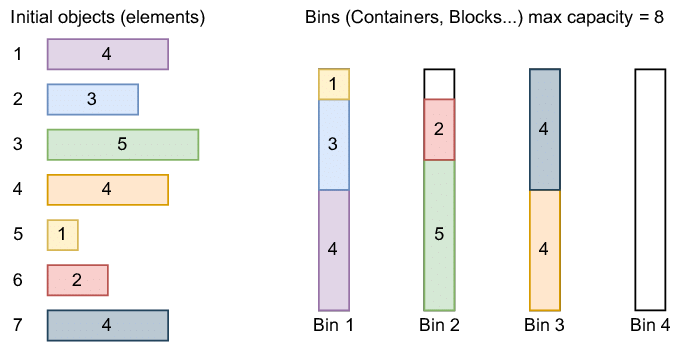
\includegraphics[width=0.5\linewidth]{Illustration-of-the-bin-packing-problem.png}
    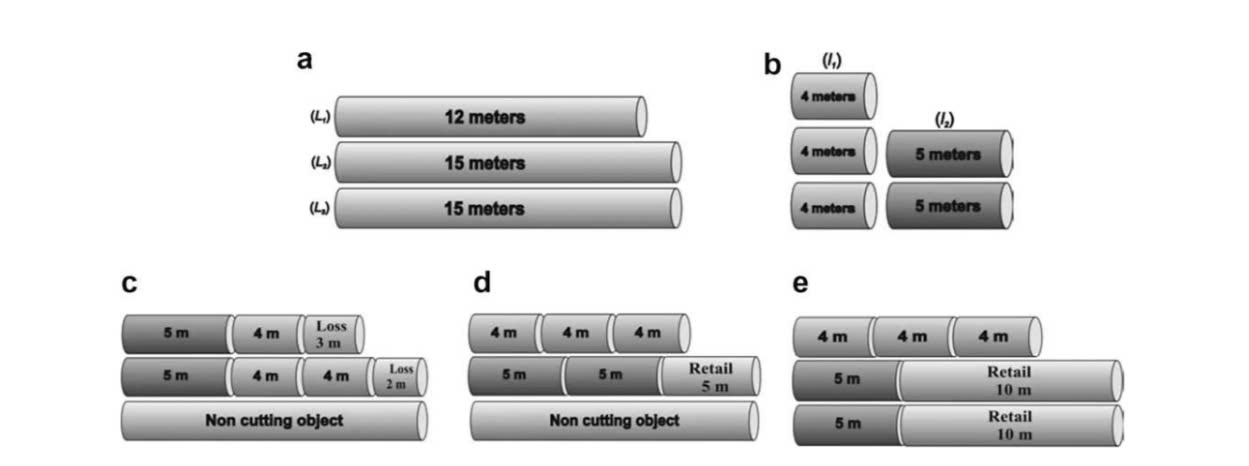
\includegraphics[width=0.5\linewidth]{pattern_generation_image.jpg}
    \caption{Mô phỏng bài toán Bin Packing (Hình trên) và Mô phỏng bài toán Cutting Stock Problem ((a) vật liệu (b) sản phẩm yêu cầu (c) - (e) các giải pháp)}
    \label{fig:enter-label}
\end{figure}
\indent Hình trên cho thấy sự tương đồng giữa bài toán \textbf{One - Dimensional Bin Packing} với việc xây dựng các mẫu cắt cho thuật toán (là bài toán \textbf{Pattern Generation}) khi ta cần sắp sếp một số loại vật thể cố định vào một khuôn mẫu nhất định và tối ưu các mẫu đó để giảm thiểu phần dư thừa nhiều nhất có thể. Chính vì thế nhóm đề xuất các thuật toán khá phổ biến khi giải quyết bài toán \textbf{One - Dimensional Bin Packing} để tối ưu \textbf{Exhaustive Repetition Heuristic - Algorithm} mà nhóm đã sử dụng.\\
%Inserting mô hinh :))))%
\indent Cụ thể ở đây là hai giải thuật sau:
\begin{itemize}
    \item Giải thuật First-Fit Decrease (FFD)
    \item Giải thuật Greedy
\end{itemize}
\subsubsection{First-Fit Decrease Algorithm}
\indent\indent Trong \textbf{\textit{Cutting Stock Problem}}, một trong những thách thức quan trọng là tối ưu hóa việc sử dụng vật liệu bằng cách tạo ra các mẫu cắt hiệu quả. Thuật toán First Fit Decreasing (FFD) là một trong những phương pháp phổ biến được sử dụng để tạo mẫu cắt. Thuật toán này được biết đến với khả năng tìm ra giải pháp hợp lý trong thời gian ngắn và dễ dàng triển khai.\\
\indent \textbf{\textit{Hướng tiếp cận}} \\
\indent Thuật toán \textbf{\textit{First Fit Decreasing (FFD)}} sắp xếp các đối tượng cần cắt (items) theo thứ tự giảm dần về kích thước, sau đó lần lượt xếp chúng vào các không gian trống (bins) có sẵn theo nguyên tắc \textit{"first fit"} (vừa khít đầu tiên). Trong ngữ cảnh bài toán cắt tấm, các đối tượng này là các kích thước của các phần tử cần cắt và các không gian trống là các tấm vật liệu có kích thước nhất định.
%INSERTING FLOWCHART :))))%
\subsubsection{Greedy Algorithm}
\indent\indent Trong \textbf{\textit{Cutting Stock Problem}}, mục tiêu chính là tối ưu hóa việc sử dụng vật liệu bằng cách tạo ra các mẫu cắt sao cho lượng phế liệu bị lãng phí là nhỏ nhất. Thuật toán Greedy là một trong những phương pháp tiếp cận cơ bản và phổ biến nhất, được sử dụng để giải quyết bài toán này. Phương pháp này đặc biệt hữu ích trong các bài toán yêu cầu giải pháp nhanh chóng và đơn giản.\\
\indent \textbf{\textit{Hướng tiếp cận}} \\
\indent Thuật toán \textbf{\textit{Greedy}} hoạt động dựa trên nguyên tắc chọn lựa cục bộ tối ưu tại mỗi bước với hy vọng rằng sự lựa chọn này sẽ dẫn đến giải pháp toàn cục tối ưu. Trong ngữ cảnh bài toán cắt tấm, tại mỗi bước, thuật toán chọn phần tử có kích thước lớn nhất hoặc phần tử dễ xếp nhất (phù hợp nhất) vào không gian trống hiện tại của tấm vật liệu.
\subsection{Mô hình 1}
\indent\indent Ở mô hình 1 nhóm sẽ xây dựng phương phảp giải quyết bài toán \textbf{CSP} theo \textbf{Exhaustive Repetition Heuristic} với \textbf{Step 1} của heuristic được tối ưu bằng thuật toán \textbf{First Fit Decrease (FFD)} \\
\indent \textbf{Flowchart} 
\begin{figure}[http]
    \centering
    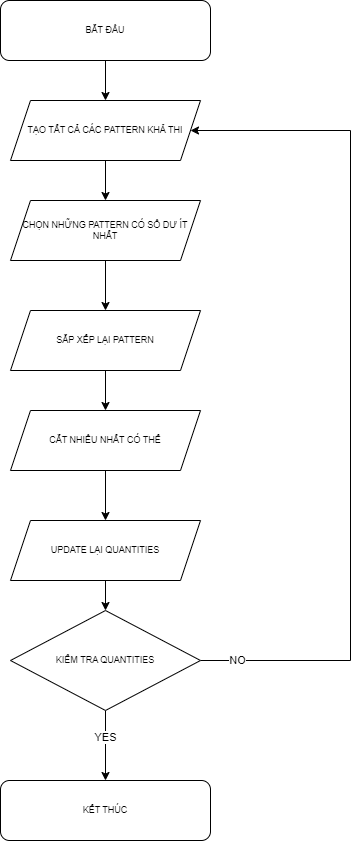
\includegraphics[width=0.2\linewidth]{FFD FLOWCHART-Page-1.drawio.png}
    \caption{Mô hình 1 flowchart}
    \label{tab:sample}
\end{figure}
\clearpage
\subsection{Mô hình 2}
\indent\indent Ở mô hình 2 nhóm sẽ xây dựng phương phảp giải quyết bài toán \textbf{CSP} theo \textbf{Exhaustive Repetition Heuristic} với \textbf{Step 1} của heuristic được tối ưu bằng thuật toán \textbf{Greedy} \\
\indent \textbf{Flowchart} 
\begin{figure}[http]
    \centering
    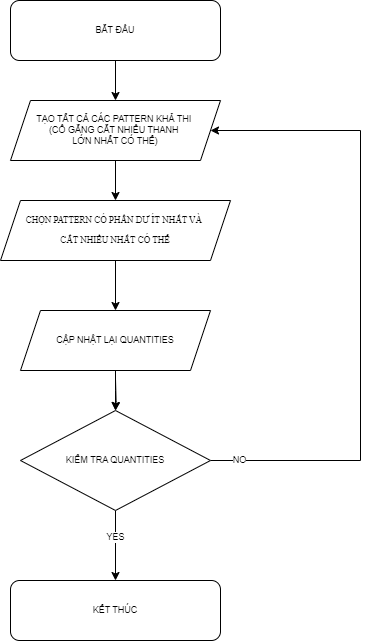
\includegraphics[width=0.2\linewidth]{FFD FLOWCHART-Trang-2.drawio.png}
    \caption{Mô hình 2 flowchart}
    \label{tab:sample}
\end{figure}
\subsection{Thiết kế chương trình thực thi giải thuật}
\indent Chương trình được nhóm hiện thực hoàn toàn bằng ngôn ngữ \textbf{Python} với đầu vào (input) và đầu ra (output) được thiết kế như sau: \\
\indent\textbf{Input:} \\
\indent Input là một file .txt với các thông số 
\begin{itemize}
    \item \indent \textbf{dòng đầu tiên} là một dãy số nguyên cách nhau bởi dấu phẩy tượng trưng cho một list độ dài của các thanh cần cắt.
    \item \indent \textbf{dòng thứ hai} là một dãy số nguyên cách nhau bởi dấu phẩy tượng trưng cho nhu cầu tương ứng của mỗi thanh so với dòng đầu tiên.
    \item \indent \textbf{dòng thứ ba} là một dãy số nguyên cách nhau bởi dấu phẩy tượng trưng cho một list các thanh được cắt
\end{itemize}
\begin{lstlisting}[language=Python,caption={Input file}]
    2, 3, 4
    6, 4, 4
    5, 6, 9    
\end{lstlisting}
\indent\textbf{Output:} 
\begin{lstlisting}[language=Python,caption={Terminal Console}]
    All patterns need to use:
    {'stock': 9, 'cuts': {0: 1, 1: 1, 2: 1}, 'leftover': 0}
    {'stock': 9, 'cuts': {0: 1, 1: 1, 2: 1}, 'leftover': 0}
    {'stock': 9, 'cuts': {0: 1, 1: 1, 2: 1}, 'leftover': 0}
    {'stock': 9, 'cuts': {0: 1, 1: 1, 2: 1}, 'leftover': 0}
    {'stock': 5, 'cuts': {0: 2, 1: 0, 2: 0}, 'leftover': 1}
    
    Summarize:
    use {'stock': 9, 'cuts': {0: 1, 1: 1, 2: 1}, 'leftover': 0} 4 times
    use {'stock': 5, 'cuts': {0: 2, 1: 0, 2: 0}, 'leftover': 1} 1 times
    
    Remaining quantities: [0, 0, 0]
    Sum of leftover: 1
    Total time: 0.0 sec
    Total stock: 5
\end{lstlisting}
\indent Output của chương trình mà nhóm đã được thiết kế thành 6 dữ kiện:
\begin{itemize}
    \item \textbf{All patterns need to use} đây là thứ tự sử dụng các pattern được chọn ra trong vùng feasible pattern để giải quyết trường hợp.
    \item  \textbf{Summarize} Thống kê lại các loại pattern đã được sử dụng
    \item \textbf{Remaining quantities} cập nhật lại demand khi chương trình đã chạy xong, list này giá trị 0 tức nghĩa chương trình đã hoàn thành demand được đề bài đưa ra.
    \item \textbf{Sum of leftover} tổng số lượng dư. 
    \item \textbf{Total time} thời gian thực thi.
    \item \textbf{Total stock} tổng số lượng các thanh đã được sử dụng(không phân biệt từng loại thanh).
\end{itemize}
\indent \textbf{Xử lý ngoại lệ:}\\
\indent Những trường hợp sau đây chương trình sẽ thông báo lỗi: \\
\indent\indent \text{-} Số lượng yêu cầu của các vật thể khác với số lượng vật thể chương trình sẽ báo lỗi sau: \textbf{Input Error: the length of item demand list are different from the lenght of item list}\\
\indent\indent \text{-} Độ dài các vật thể yêu cầu lớn hơn so với các vật liệu được cắt chương trình sẽ báo lỗi sau: \textbf{Input Error: One or more item is longer than the maximum length of the stock.}

   
   
   




\section{Mô hình hóa vấn đề}
\subsection{Phân tích vấn đề}
\indent \indent Trong hầu hết các ngành công nghiệp, chi phí nguyên liệu chiếm tỷ lệ cao trong tổng giá thành (hơn 80\%). Bài toán cắt nguyên liệu (CSP) là một trong những bài toán nổi tiếng trong nghiên cứu hoạt động, được định nghĩa nhằm cải thiện chất lượng sử dụng nguyên liệu. Bài toán CSP này có thể được mô tả như sau: Có một tập hợp các vật liệu hình chữ nhật với các chiều rộng khác nhau (nhưng có cùng chiều dài \textbf{\textit{L}}) và chúng ta sẽ chia chúng thành các mảnh nhỏ hơn có chiều rộng mong muốn (với cùng chiều dài \textbf{\textit{L}}).\\
\indent Trước tiên, các chiều rộng mong muốn được sắp xếp theo thứ tự giảm dần $(w_{1}, w_{2},...)$ và sau đó chia các vật liệu ban đầu thành các mảnh nhỏ có chiều rộng $w_{1}$ nhiều nhất có thể. Nếu còn lại phần nguyên liệu thừa, ta tiếp tục với chiều rộng mong muốn tiếp theo $w_{2}$ và chia phần thừa đó thành các mảnh nhỏ có chiều rộng $w_{2}$. Bằng cách tiếp tục quy trình tương tự cho đến chiều rộng nhỏ nhất yêu cầu, ta có thể tạo ra tất cả các mẫu cắt và cuối cùng tính toán phần thừa nguyên liệu tối thiểu.\\
\indent Đặc biệt đối với cách tiếp cận lần này trường hợp sẽ đơn giản hơn do sẽ không có ràng buộc về số lượng thanh được sử dụng hoặc số lượng dư thừa tối đa, tuy nhiên mô hình bài toán cũng phải đáp ứng được việc giải quyết các vấn đề khi có nhiều hơn 1 vật liệu.
% Thêm hình ảnh và ví dụ mô phỏng cho bài toán
\subsection{Mô hình bài toán}
\subsubsection{Hệ thống ký hiệu}
 \begin{table}[h]
        \centering
        \begin{tabular}{ll}    
        \hline \hline
        Ký hiệu     & Định nghĩa \\ \hline \hline
        $h$     & Số loại vật liệu được cắt (với các kích cỡ khác nhau) \\
        $n$     & Số lượng các vật thể yêu cầu \\
        $m$     & Số lượng mẫu \\
        $a_{ikj}$     & Số lần xuất hiện vật thể thứ i trên vật liệu thứ k trong mẫu thứ j \\
        $c_{kj}$     & Hệ số chi phí (hoặc hệ số tương tự) liên quan đến việc sử dụng mẫu\\ cắt thứ j cho vật liệu loại k. \\
        $d_{i}$     & Yêu cầu của vật thể thứ i \\
        \hline
        $x_{kj}$     &  Số lần mẫu cắt thứ j của vật liệu loại k được sử dụng.\\    
        \hline \hline
        \end{tabular}
        \caption{Hệ thống các ký hiệu}
        \label{Symbol}
    \end{table}
\subsubsection{Hàm mục tiêu}
\indent \indent Mục tiêu chính của chúng ta đối với mô hình bài toán này là tối thiểu hóa tổng lãng phí khi ta sử dụng các mẫu cắt. Đây là một trong nhiều cách dùng để mô hình hóa bài toán trên, chúng ta có thể thay thế hàm mục tiêu bằng việc tối thiểu hóa số lượng mẫu cắt được sử dụng thay vì tối thiểu tổng số lãng phí khi ta sử dụng các mẫu cắt. Tuy nhiên, ở đây nhóm quyết định chọn hướng mô hình hóa với mục tiêu tối thiểu hóa tổng số lượng lãng phí. \\
\begin{equation}
    \text{Min} \sum_{k = 1}^{h}\sum_{j = 1}^{m} c_{kj}.x_{kj} \text{ (Total Cutloss)}
\end{equation}
\indent Với $x_{kj}$ là số lần mẫu cắt thứ j của vật liệu loại k được sử dụng và $c_{kj}$ Tổn thất trong mẫu thứ j vật liệu loại k, vì vậy tích $x_{kj}.c_{kj}$ chính là tổng tổn thất của của mẫu thứ j của vật liệu loại k.
\subsubsection{Các ràng buộc}
\subsubsection{Ràng buộc về nhu cầu}
\indent\indent Đây là ràng buộc nhu cầu, đảm bảo rằng tổng số vật thể \textbf{\textit{i}} được cắt từ tất cả các vật liệu theo các mẫu khác nhau phải lớn hơn hoặc bằng nhu cầu \textbf{\textit{$d_{i}$}} của vật thể đó.
\begin{equation}
    \sum_{k = 1}^{h}\sum_{j = 1}^{m} a_{ikj}.x_{kj} \geq d_{i}, \text{ i = 1,... m}
\end{equation}
\subsubsection{Ràng buộc về giới hạn vật liệu}
\indent \indent Ràng buộc này là phần mở rộng thêm, tuy nhiên trong nghiên cứu của nhóm sẽ các giải thuật và heuristic được xây dựng sẽ không giải quyết vấn đề có chứa ràng buộc này.
\begin{equation}
    \sum_{j = 1}^{m} \leq e_{k}, \text{ k = 1, 2,... h}
\end{equation}
\indent Ràng buộc này sẽ đảm bảo số lượng vật liệu \textbf{\textit{k}} được cắt theo mẫu \textbf{\textit{j}} sẽ không vượt quá số lượng vật liệu \textbf{\textit{k}} có sẵn.
\subsubsection{Ràng buộc nguyên và không âm}
\indent\indent Ràng buộc để đảm bảo biến quyết định $x_{jk}$ và biến $c_{jk}$ của hàm mục tiêu phải là số nguyên và không âm. 
\begin{equation}
    \begin{cases}
        x_{jk} \geq 0 \\
        c_{jk} \geq 0  
    \end{cases}
    , \text{ j = 1, 2,... m; k = 1, 2,... h}
\end{equation}



\section{Phân tích kết quả thực thi mô hình trên các bộ dữ liệu}
\indent\indent Ở phần này nhóm sẽ đánh giá các mô hình để giải bài toán bằng các giải thuật và heuristic đã trình bài ở trên thông qua hai phần, phần 1 sẽ đánh giá và so sánh kết quả giữa hai mô hình mà nhóm đã xây dựng dựa trên bộ dữ liệu tự tạo của các nhà nghiên cứu đi trước đồng thời sẽ so sánh hiệu quả của giải thuật mà nhóm nghiên cứu với các giải thuật mà các nhà nghiên cứu trước đã xây dựng trên cùng một bộ dữ liệu, phần 2 nhóm sẽ áp dụng các mô hình đã xây dựng được vào một case-study thực tế và đánh giá khả năng ứng dụng của mô hình.
\subsection{The Case Study (Real World Data)}
\subsubsection{Mô tả trường hợp}
\indent\indent Để minh họa tính ứng dụng của mô hình mà nhóm đã phát triển, nghiên cứu trường hợp liên quan đến vấn đề cắt gặp phải tại một công ty sản xuất pallet gỗ quy mô vừa và nhỏ (SME) ở Thái Lan sẽ được trình bày và thảo luận.\\
\indent Gỗ thông được nhập khẩu từ New Zealand, vận chuyển dưới dạng container. Gỗ thông nhập khẩu được cắt thành các thanh hình chữ nhật tiêu chuẩn có kích thước 150 × 100 mm với các độ dài (Lk) lần lượt là 4,2 m, 4,8 m, 5,4 m, và 6,0 m một cách ngẫu nhiên. Chi phí trung bình của gỗ thông nhập khẩu (bao gồm cả chi phí vận chuyển) là 265 Baht/foot³. Gỗ thông phải được cắt thành các sản phẩm có kích thước yêu cầu tùy thuộc vào mẫu pallet cần sản xuất. Độ dài của mỗi sản phẩm (li) được thể hiện trong Bảng bên dưới.
\begin{figure}[http]
    \centering
    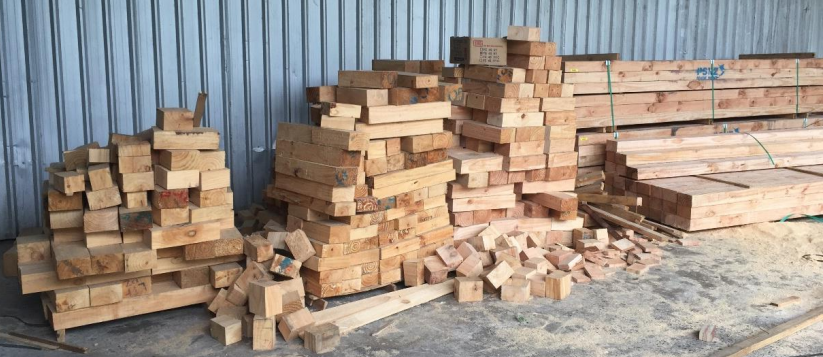
\includegraphics[width=0.7\linewidth]{CaseStudyPicture.png}
    \caption{Tấm gỗ(Stock) và phần dư thừa của nó(off-cuts)}
    \label{tab:sample}
\end{figure}
\begin{table}[http]
\centering
\begin{tabular}{c|ccccccc}
  \textbf{\textit{Item (mm)}} & 2316 & 2200 & 1650 & 1460 &  1140 & 1120 & 980 \\
  \hline
  \textbf{\textit{Demand}} & 789 & 254 & 468 & 554 & 4686 & 1179 & 969 \\
\end{tabular}
\caption{Bảng nhu cầu của Case Study}
\label{tab:sample}
\end{table}

\subsubsection{Kết quả thực thi}
\indent\indent Kết quả sau khi chạy \textbf{\textit{mô hình 1}} để giải quyết \textbf{\textit{Case-Study}} trên như sau:
\begin{lstlisting}[language=Python,caption={Terminal Console}]
    Remaining quantities: [0, 0, 0, 0, 0, 0, 0]
    Sum of leftover: 361296
    Total time: 0.015075445175170898 sec
    Total stock: 2448
\end{lstlisting}

\indent Kết quả sau khi chạy \textbf{\textit{mô hình 2}} để giải quyết \textbf{\textit{Case-Study}} trên như sau:
\begin{lstlisting}[language=Python,caption={Terminal Console}]
    Remaining quantities: [0, 0, 0, 0, 0, 0, 0]
    Sum of leftover: 475896
    Total time (greedy): 0.003785848617553711 sec
    Total stock (greedy): 2452
\end{lstlisting}


\begin{table}[http]
    \centering
    \small
    \begin{tabular}{|c|c|c|c|c|c|c|c|c|}
    \hline
    \multirow{2}{*}{\textbf{\begin{tabular}[c]{@{}c@{}}Stock\\ length (mm)\end{tabular}}} & \multirow{2}{*}{\textbf{\begin{tabular}[c]{@{}c@{}}Required pattern\\ (piece)\end{tabular}}} & \multicolumn{7}{c|}{\textbf{No. of item to be cut with the length of (mm)}} \\ \cline{3-9} 
     &  & \textbf{2316} & \textbf{2200} & \textbf{1650} & \textbf{1460} & \textbf{1140} & \textbf{1120} & \textbf{980} \\ \hline
     \multirow{1}{*}{4200} & 217 & 0 & 0 & 0 & 0 & 0 & 2 & 2 \\ \hline
    \hline
    \multirow{7}{*}{4800} & 254 & 0 & 1 & 0 & 1 & 1 & 0 & 0 \\ \cline{2-9} 
     & 394 & 2 & 0 & 0 & 0 & 0 & 0 & 0 \\ \cline{2-9} 
     & 1 & 1 & 0 & 0 & 0 & 2 & 0 & 0 \\ \cline{2-9} 
     & 1107 & 0 & 0 & 0 & 0 & 4 & 0 & 0 \\ \cline{2-9} 
     & 1 & 0 & 0 & 0 & 0 & 2 & 2 & 0 \\ \cline{2-9} 
     & 89 & 0 & 0 & 0 & 0 & 0 & 4 & 0 \\ \cline{2-9} 
     & 1 & 0 & 0 & 0 & 0 & 0 & 3 & 1 \\ \hline
     \hline     
    \multirow{1}{*}{5400} & 234 & 0 & 0 & 2 & 0 & 0 & 1 & 1 \\ \hline
    \hline
    \multirow{1}{*}{6000} & 150 & 0 & 0 & 0 & 2 & 0 & 1 & 2 \\ 
    \hline \hline     
    \multicolumn{2}{|c|}{\textbf{Number of each item}} & 789 & 254 & 468 & 554 & 4686 & 1179 & 969 \\ \hline
    \end{tabular}
    \caption{Kế hoạch cắt các thanh gỗ được tạo ra bởi mô hình 1}
    \label{table:cutting_plan}
\end{table}
\begin{table}[http]
    \centering
    \small
    \begin{tabular}{|c|c|c|c|c|c|c|c|c|}
    \hline
    \multirow{2}{*}{\textbf{\begin{tabular}[c]{@{}c@{}}Stock\\ length (mm)\end{tabular}}} & \multirow{2}{*}{\textbf{\begin{tabular}[c]{@{}c@{}}Required pattern\\ (piece)\end{tabular}}} & \multicolumn{7}{c|}{\textbf{No. of item to be cut with the length of (mm)}} \\ \cline{3-9} 
     &  & \textbf{2316} & \textbf{2200} & \textbf{1650} & \textbf{1460} & \textbf{1140} & \textbf{1120} & \textbf{980} \\ \hline
     \multirow{3}{*}{4200} & 1 & 0 & 0 & 1 & 1 & 0 & 0 & 1 \\ \cline{2-9} 
     & 1 & 0 & 0 & 0 & 0 & 0 & 1 & 3 \\ \cline{2-9} 
     & 1 & 0 & 0 & 0 & 0 & 0 & 0 & 1 \\ \cline{2-9} 
     \hline
    \hline
    \multirow{5}{*}{4800} & 394 & 2 & 0 & 0 & 0 & 0 & 0 & 0 \\ \cline{2-9} 
     & 233 & 0 & 0 & 2 & 1 & 0 & 0 & 0 \\ \cline{2-9} 
     & 1171 & 0 & 0 & 0 & 0 & 4 & 0 & 0 \\ \cline{2-9} 
     & 1 & 0 & 0 & 0 & 0 & 2 & 2 & 0 \\ \cline{2-9} 
     & 294 & 0 & 0 & 0 & 0 & 0 & 4 & 0 \\ \cline{2-9} 
     \hline
     \hline     
    \multirow{3}{*}{5400} & 126 & 0 & 2 & 0 & 0 & 0 & 0 & 1 \\ \cline{2-9} 
    & 1 & 0 & 1 & 1 & 1 & 0 & 0 & 0 \\ \cline{2-9} 
    & 106 & 0 & 0 & 0 & 3 & 0 & 0 & 1 \\ \cline{2-9} 
    \hline
    \hline
    \multirow{1}{*}{6000} & 1 & 1 & 1 & 0 & 1 & 0 & 0 & 0 \\ \cline{2-9} 
    & 122 & 0 & 0 & 2 & 1 & 0 & 0 & 6 \\ 
    \hline \hline     
    \multicolumn{2}{|c|}{\textbf{Number of each item}} & 789 & 254 & 712 & 676 & 4686 & 1179 & 969 \\ \hline
    \end{tabular}
    \caption{Kế hoạch cắt các thanh gỗ được tạo ra bởi mô hình 2}
    \label{table:cutting_plan}
\end{table}

\subsubsection{Kết luận}
\begin{table}[h]
    \centering
    \small
    \caption{So sánh hai mô hình}
    \label{tab:cutting_plans}
    \begin{tabular}{|l|c|c|c|}        
        \hline        
        & Mô hình 1 & Mô hình 2 & Change \\
        \hline        
        Volume of stock required (foot$^3$) & 6,327.42  & 6,379.2 & -51.78 \\
        \hline        
        Cost of stock (Baht/$foot^3$) & 1,676,766.3 & 1,690,488 & -13721.7 \\
        \hline
        Volume of waste (foot$^3$) & 191.31 & 252.16 & -60.85 \\
        \hline        
        Cost of waste (Baht/$foot^3$) & 50,697 & 66,822.4 & -16,125.25  \\
        \hline        
    \end{tabular}
\end{table}
\indent Nhìn chung đối với bài toán này ta sử dụng Mô hình 1 với cách tối ưu bằng thuật toán FFD sẽ là giải pháp tốt hơn so với Mô hình 1 tối ưu bằng thuật toán Greedy. \\
\indent \textbf{\textit{Về thời gian thực thi:}} sự chênh lệch thời gian thực thi của hai mô hình trên là không đáng kế, việc này sẽ không ảnh hưởng gì khi áp dụng vào thực tế, tuy nhiên trong trường hợp này thời gian thực thi của mô hình 2 lại có phần nhỉnh hơn. \\
\indent \textbf{\textit{Về việc áp dụng thực tế:}} Khi xét về mặt dư thừa và chi phí mô hình 2 sẽ tốt hơn so với mô hình 1, nhưng nếu xét về khía cạnh môi trường thì doanh nghiệp có thể sẽ ưu tiên sử dụng mô hình 1 do dựa trên kết quả khi thực thi trên máy tính thì \textbf{\textit{Total stock}} của mô hình 1 ít hơn so với mô hình 2 4 thanh. Việc chênh lệch như vậy sẽ giảm bớt việc tiêu thụ điện năng, việc khai thác gỗ sử dụng, việc vận chuyển các thanh  nguyên liệu. \\
\indent \textbf{\textit{So sánh với giải pháp của một vài nhà nghiên cứu:}} Ở đây nhóm sẽ so sánh với nhóm nghiên cứu của P Wattanasiriseth A Krairit [4] cũng thực hiện nghiên cứu trên Case Study tương tự, nhưng tiếp cận vấn đề với một phương pháp khác. Cụ thể, nhóm nghiên cứu sau giải quyết Case-Study bằng \textbf{Giải thuật Cutting Plan} và \textbf{Giải thuật Optimal Cutting Plan}. Kết quả đạt được của nhóm được thể hiện như sau:
\begin{figure}[http]
    \centering
    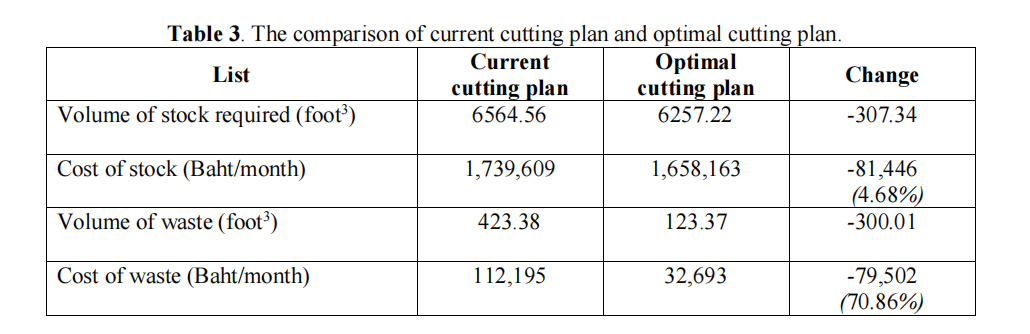
\includegraphics[width=1\linewidth]{CuttingPlans.png}
    \caption{Tiếp cận Case Study bằng giải thuật Cutting Plans}
    \label{fig:enter-label}
\end{figure}
\\
\indent Dựa theo kết quả của nhóm nghiên cứu trên thì thuật toán Cutting Plans có thể dễ dàng nhận thấy kém hiệu quả hơn so với Mô hình 1 và Mô hình 2 mà nhóm đã xây dựng.



\subsection{Synthetic Data}
\indent\indent Mặc dù có nhiều tài liệu phong phú về CSPs, rất ít người cung cấp dữ liệu thực tế cho các bài toán của họ. So sánh trực tiếp với họ là rất khó, nếu không muốn nói là không thể. Trong các nghiên cứu thực nghiệm của nhóm, 10 bài toán thử nghiệm được sử dụng (mười bài toán chuẩn được lấy từ Hinterdingand Khan [1]). Mô tả chi tiết về các bài toán này được cung cấp bên dưới. Tổng số mục được yêu cầu thay đổi từ 20 đến 126. Các bài toán 1-5 là các bài toán CSP có nhiều độ dài vật liệu và các bài toán 1a đến 5a là các bài toán CSP có một độ dài tấm. Các bài toán có cùng chỉ số có cùng số lượng mục được yêu cầu, ví dụ như các bài toán 4 và 4a có cùng số lượng mục được yêu cầu.
\begin{table}[http]
    \centering
    \small
    \caption{The benchmark problems}
    \label{tab:benchmark}
    \begin{tabular}{lccccccccccc}
        \hline
        \\
        Problem 1: 10, 13, 15 \\
        Problem 1a: 14 & \multicolumn{8}{c}{20 items} \\
        \toprule
        Item length & 3 & 4 & 5 & 6 & 7 & 8 & 9 & 10 \\
        No. required & 5 & 2 & 1 & 2 & 4 & 2 & 1 & 3 \\
        \midrule
        \\
        \hline
        \\
        Problem 2: 10, 13, 15  \\
        Problem 2a: 15 & \multicolumn{8}{c}{50 items} \\
        \toprule
        Item length & 3 & 4 & 5 & 6 & 7 & 8 & 9 & 10 \\
        No. required & 4 & 8 & 5 & 7 & 8 & 5 & 5 & 8 \\
        \midrule
        \\
        \hline
        \\
        Problem 3: 10, 13, 15, 20, 22, 25 \\
        Problem 3a: 25 & \multicolumn{8}{c}{60 items} \\
        \toprule
        Item length & 3 & 4 & 5 & 6 & 7 & 8 & 9 & 10 \\
        No. required & 6 & 12 & 6 & 5 & 15 & 6 & 4 & 6 \\
        \midrule
        \\
        \hline
        \\
        Problem 4: 13, 20, 25 \\
        Problem 4a: 25 & \multicolumn{8}{c}{60 items} \\
        \toprule
        Item length & 3 & 4 & 5 & 6 & 7 & 8 & 9 & 10 \\
        No. required & 7 & 12 & 15 & 7 & 4 & 6 & 8 & 1 \\
        \hline
        \midrule                
        \bottomrule
    \end{tabular}      
    \begin{tabular}{lcccccccccc}
        \\
        \hline
        \\
        \toprule
        \multicolumn{11}{l}{Problem 5: 4300, 4250, 4150, 3950, 3800, 3700, 3550, 3500} \\
        \multicolumn{11}{l}{Problem 5a: 4300 \quad 126 items} \\
        \midrule
        Item length & 2350 & 2250 & 2200 & 2100 & 2050 & 2000 & 1950 & 1900 & 1850 & 1700 \\
        No. required & 2 & 4 & 4 & 15 & 6 & 11 & 6 & 15 & 13 & 5 \\
        Item length & 1650 & 1350 & 1300 & 1250 & 1200 & 1150 & 1100 & 1050 & - & - \\
        No. required & 2 & 9 & 3 & 6 & 10 & 4 & 8 & 3 & - & - \\
        \bottomrule
        \\
        \hline
        \\
        \toprule
        \multicolumn{11}{l}{Problem 6: 86, 83, 79, 76, 72} \\
        \multicolumn{11}{l}{Problem 6a: 86 \quad 200 items} \\
        \midrule
        Item length & 21 & 23 & 24 & 25 & 26 & 27 & 28 & 29 & 31 & - \\ %thêm 1 cột%
        No. required & 10 & 14 & 10 & 7 & 14 & 4 & 13 & 9 & 5 & - \\
        Item length & 33 & 34 & 35 & 37 & 38 & 41 & 42 & 44 & 47 & - \\
        No. required & 10 & 13 & 10 & 11 & 15 & 12 & 15 & 15 & 13 & - \\
        \toprule
        \\
        \hline        
        \bottomrule
    \end{tabular}        
    % \begin{tabular}{lcccccccccccc}
    %     \\
    %     \hline
    %     \\
    %     \multicolumn{13}{l}{Problem 7: 120, 115, 110, 105, 100} \\
    %     \multicolumn{13}{l}{Problem 7a: 120 \quad 200 items} \\
    %     \midrule
    %     Item length & 22 & 26 & 27 & 28 & 29 & 30 & 31 & 32 & 34 & 36 & 37 & 38 \\
    %     No. required & 12 & 8 & 27 & 15 & 25 & 7 & 10 & 22 & 5 & 16 & 19 & 21 \\
    %     Item length & 39 & 46 & 47 & 48 & 52 & 53 & 54 & 56 & 58 & 60 & 63 & 64 \\
    %     No. required & 26 & 16 & 12 & 26 & 20 & 25 & 9 & 17 & 22 & 14 & 17 & 9 \\
    %     \\
    %     \hline
    %     \\
    %     \toprule
    %     \multicolumn{13}{l}{Problem 8: 120, 115, 110} \\
    %     \multicolumn{13}{l}{Problem 8a: 120 \quad 400 items} \\
    %     \midrule
    %     Item length & 22 & 23 & 24 & 26 & 27 & 28 & 29 & 30 & 31 & 36 & 39 & 41 \\ %thêm 1 cột%
    %     No. required & 12 & 8 & 27 & 15 & 25 & 7 & 10 & 22 & 5 & 16 & 19 & 21 \\
    %     Item length & 42 & 48 & 49 & 50 & 51 & 54 & 55 & 56 & 59 & 60 & 66 & 67 \\
    %     No. required & 26 & 16 & 12 & 26 & 20 & 25 & 9 & 17 & 22 & 14 & 17 & 9 \\
    %     \toprule
    %     \\
    %     \hline
    %     \\
    %     \multicolumn{13}{l}{Problem 9: 120, 115, 110, 105, 100} \\
    %     \multicolumn{13}{l}{Problem 9a: 120 \quad 400 items} \\
    %     \midrule
    %     Item length & 21 & 22 & 24 & 25 & 27 & 29 & 30 & 31 & 32 & 33 & 34 & 35 \\
    %     No. required & 13 & 15 & 7 & 5 & 9 & 9 & 3 & 15 & 18 & 17 & 4 & 17 \\
    %     Item length & 38 & 39 & 42 & 44 & 45 & 46 & 47 & 48 & 49 & 50 & 51 & 52 \\
    %     No. required & 20 & 9 & 4 & 19 & 9 & 12 & 15 & 3 & 20 & 14 & 15 & 6 \\
    %     Item length & 53 & 54 & 55 & 56 & 57 & 59 & 60 & 61 & 63 & 65 & 66 & 67 \\
    %     No. required & 4 & 7 & 5 & 19 & 19 & 6 & 3 & 7 & 20 & 5 & 10 & 7 \\
    %     \\
    %     \hline
    %     \\
    %     \toprule
    %     \multicolumn{13}{l}{Problem 10: 120, 115, 110} \\
    %     \multicolumn{13}{l}{Problem 10a: 120 \quad 600 items} \\
    %     \midrule
    %     Item length & 21 & 22 & 23 & 24 & 27 & 28 & 29 & 30 & 31 & 33 & 35 \\
    %     No. required & 13 & 19 & 24 & 20 & 23 & 24 & 15 & 5 7 24 & 16 & 12 & 24 \\
    %     Item length & 36 & 39 & 40 & 41 & 42 & 43 & 44 & 45 & 46 & 47 & 48 & 50 \\
    %     No. required & 16 & 4 & 20 & 24 & 6 & 14 & 21 & 20 & 24 & 2 & 11 & 26 \\
    %     Item length & 51 & 54 & 56 & 57 & 58 & 61 & 62 & 63 & 64 & 65 & 66 & 67 \\
    %     No. required & 23 & 25 & 8 &16 & 10 & 14 & 6 & 19 & 18 & 11 & 27 & 16 \\
    %     \toprule
    %     \\
    %     \hline
    %     \\
    %     \bottomrule
    % \end{tabular}    
\end{table}

\begin{table}[http]
    \centering
    \small
    \begin{tabular}{lcccccccccccc}
        \\
        \hline
        \\
        \multicolumn{13}{l}{Problem 7: 120, 115, 110, 105, 100} \\
        \multicolumn{13}{l}{Problem 7a: 120 \quad 200 items} \\
        \midrule
        Item length & 22 & 26 & 27 & 28 & 29 & 30 & 31 & 32 & 34 & 36 & 37 & 38 \\
        No. required & 12 & 8 & 27 & 15 & 25 & 7 & 10 & 22 & 5 & 16 & 19 & 21 \\
        Item length & 39 & 46 & 47 & 48 & 52 & 53 & 54 & 56 & 58 & 60 & 63 & 64 \\
        No. required & 26 & 16 & 12 & 26 & 20 & 25 & 9 & 17 & 22 & 14 & 17 & 9 \\
        \\
        \hline
        \\
        \toprule
        \multicolumn{13}{l}{Problem 8: 120, 115, 110} \\
        \multicolumn{13}{l}{Problem 8a: 120 \quad 400 items} \\
        \midrule
        Item length & 22 & 23 & 24 & 26 & 27 & 28 & 29 & 30 & 31 & 36 & 39 & 41 \\ %thêm 1 cột%
        No. required & 12 & 8 & 27 & 15 & 25 & 7 & 10 & 22 & 5 & 16 & 19 & 21 \\
        Item length & 42 & 48 & 49 & 50 & 51 & 54 & 55 & 56 & 59 & 60 & 66 & 67 \\
        No. required & 26 & 16 & 12 & 26 & 20 & 25 & 9 & 17 & 22 & 14 & 17 & 9 \\
        \toprule
        \\
        \hline
        \\
        \multicolumn{13}{l}{Problem 9: 120, 115, 110, 105, 100} \\
        \multicolumn{13}{l}{Problem 9a: 120 \quad 400 items} \\
        \midrule
        Item length & 21 & 22 & 24 & 25 & 27 & 29 & 30 & 31 & 32 & 33 & 34 & 35 \\
        No. required & 13 & 15 & 7 & 5 & 9 & 9 & 3 & 15 & 18 & 17 & 4 & 17 \\
        Item length & 38 & 39 & 42 & 44 & 45 & 46 & 47 & 48 & 49 & 50 & 51 & 52 \\
        No. required & 20 & 9 & 4 & 19 & 9 & 12 & 15 & 3 & 20 & 14 & 15 & 6 \\
        Item length & 53 & 54 & 55 & 56 & 57 & 59 & 60 & 61 & 63 & 65 & 66 & 67 \\
        No. required & 4 & 7 & 5 & 19 & 19 & 6 & 3 & 7 & 20 & 5 & 10 & 7 \\
        \\
        \hline
        \\
        \toprule
        \multicolumn{13}{l}{Problem 10: 120, 115, 110} \\
        \multicolumn{13}{l}{Problem 10a: 120 \quad 600 items} \\
        \midrule
        Item length & 21 & 22 & 23 & 24 & 27 & 28 & 29 & 30 & 31 & 33 & 35 \\
        No. required & 13 & 19 & 24 & 20 & 23 & 24 & 15 & 5 7 24 & 16 & 12 & 24 \\
        Item length & 36 & 39 & 40 & 41 & 42 & 43 & 44 & 45 & 46 & 47 & 48 & 50 \\
        No. required & 16 & 4 & 20 & 24 & 6 & 14 & 21 & 20 & 24 & 2 & 11 & 26 \\
        Item length & 51 & 54 & 56 & 57 & 58 & 61 & 62 & 63 & 64 & 65 & 66 & 67 \\
        No. required & 23 & 25 & 8 &16 & 10 & 14 & 6 & 19 & 18 & 11 & 27 & 16 \\
        \toprule
        \\
        \hline
        \\
        \bottomrule
    \end{tabular}    
    \caption{Caption}
    \label{tab:my_label}
\end{table}

% \clearpage
% \begin{table}[http]
%     \centering
%     \caption{The benchmark problems}
%     \label{tab:benchmark}
%     \begin{tabular}{lcccccccccc}
%         \hline
%         \\
%         \toprule
%         \multicolumn{11}{l}{Problem 5: 4300, 4250, 4150, 3950, 3800, 3700, 3550, 3500} \\
%         \multicolumn{11}{l}{Problem 5a: 4300 \quad 126 items} \\
%         \midrule
%         Item length & 2350 & 2250 & 2200 & 2100 & 2050 & 2000 & 1950 & 1900 & 1850 & 1700 \\
%         No. required & 2 & 4 & 4 & 15 & 6 & 11 & 6 & 15 & 13 & 5 \\
%         Item length & 1650 & 1350 & 1300 & 1250 & 1200 & 1150 & 1100 & 1050 & - & - \\
%         No. required & 2 & 9 & 3 & 6 & 10 & 4 & 8 & 3 & - & - \\
%         \bottomrule
%         \\
%         \hline
%         \\
%         \toprule
%         \multicolumn{11}{l}{Problem 6: 86, 83, 79, 76, 72} \\
%         \multicolumn{11}{l}{Problem 6a: 86 \quad 200 items} \\
%         \midrule
%         Item length & 21 & 23 & 24 & 25 & 26 & 27 & 28 & 29 & 31 & - \\ %thêm 1 cột%
%         No. required & 10 & 14 & 10 & 7 & 14 & 4 & 13 & 9 & 5 & - \\
%         Item length & 33 & 34 & 35 & 37 & 38 & 41 & 42 & 44 & 47 & - \\
%         No. required & 10 & 13 & 10 & 11 & 15 & 12 & 15 & 15 & 13 & - \\
%         \toprule
%         \\
%         \hline
%         \\
%         \bottomrule
%     \end{tabular}
% \end{table}
% \clearpage
% \begin{table}[http]
%     \centering
%     \begin{tabular}{lcccccccccccc}
%         \multicolumn{13}{l}{Problem 7: 120, 115, 110, 105, 100} \\
%         \multicolumn{13}{l}{Problem 7a: 120 \quad 200 items} \\
%         \midrule
%         Item length & 22 & 26 & 27 & 28 & 29 & 30 & 31 & 32 & 34 & 36 & 37 & 38 \\
%         No. required & 12 & 8 & 27 & 15 & 25 & 7 & 10 & 22 & 5 & 16 & 19 & 21 \\
%         Item length & 39 & 46 & 47 & 48 & 52 & 53 & 54 & 56 & 58 & 60 & 63 & 64 \\
%         No. required & 26 & 16 & 12 & 26 & 20 & 25 & 9 & 17 & 22 & 14 & 17 & 9 \\
%         \\
%         \hline
%         \\
%         \toprule
%         \multicolumn{13}{l}{Problem 8: 120, 115, 110} \\
%         \multicolumn{13}{l}{Problem 8a: 120 \quad 400 items} \\
%         \midrule
%         Item length & 22 & 23 & 24 & 26 & 27 & 28 & 29 & 30 & 31 & 36 & 39 & 41 \\ %thêm 1 cột%
%         No. required & 12 & 8 & 27 & 15 & 25 & 7 & 10 & 22 & 5 & 16 & 19 & 21 \\
%         Item length & 42 & 48 & 49 & 50 & 51 & 54 & 55 & 56 & 59 & 60 & 66 & 67 \\
%         No. required & 26 & 16 & 12 & 26 & 20 & 25 & 9 & 17 & 22 & 14 & 17 & 9 \\
%         \toprule
%         \\
%         \hline
%         \\
%         \multicolumn{13}{l}{Problem 9: 120, 115, 110, 105, 100} \\
%         \multicolumn{13}{l}{Problem 9a: 120 \quad 400 items} \\
%         \midrule
%         Item length & 21 & 22 & 24 & 25 & 27 & 29 & 30 & 31 & 32 & 33 & 34 & 35 \\
%         No. required & 13 & 15 & 7 & 5 & 9 & 9 & 3 & 15 & 18 & 17 & 4 & 17 \\
%         Item length & 38 & 39 & 42 & 44 & 45 & 46 & 47 & 48 & 49 & 50 & 51 & 52 \\
%         No. required & 20 & 9 & 4 & 19 & 9 & 12 & 15 & 3 & 20 & 14 & 15 & 6 \\
%         Item length & 53 & 54 & 55 & 56 & 57 & 59 & 60 & 61 & 63 & 65 & 66 & 67 \\
%         No. required & 4 & 7 & 5 & 19 & 19 & 6 & 3 & 7 & 20 & 5 & 10 & 7 \\
%         \\
%         \hline
%         \\
%         \toprule
%         \multicolumn{13}{l}{Problem 10: 120, 115, 110} \\
%         \multicolumn{13}{l}{Problem 10a: 120 \quad 600 items} \\
%         \midrule
%         Item length & 21 & 22 & 23 & 24 & 27 & 28 & 29 & 30 & 31 & 33 & 35 \\
%         No. required & 13 & 19 & 24 & 20 & 23 & 24 & 15 & 5 7 24 & 16 & 12 & 24 \\
%         Item length & 36 & 39 & 40 & 41 & 42 & 43 & 44 & 45 & 46 & 47 & 48 & 50 \\
%         No. required & 16 & 4 & 20 & 24 & 6 & 14 & 21 & 20 & 24 & 2 & 11 & 26 \\
%         Item length & 51 & 54 & 56 & 57 & 58 & 61 & 62 & 63 & 64 & 65 & 66 & 67 \\
%         No. required & 23 & 25 & 8 &16 & 10 & 14 & 6 & 19 & 18 & 11 & 27 & 16 \\
%         \toprule
%         \\
%         \hline
%         \\
%         \bottomrule
%     \end{tabular}    
% \end{table}
\clearpage
\subsubsection{Kết quả thực thi}
\indent Với bảng dữ liệu trên, từ problem 1 - 10 sẽ là dạng \textbf{Multiple Stock} và từ problem 1a - 10a sẽ là dạng \textbf{Single Stock}.

\begin{table}[h]
\centering
\small
\begin{tabular}{@{}l|ccc|ccc@{}}
\toprule
& \multicolumn{3}{c|}{Exhaustive Repetion Heuristic with FFD} & \multicolumn{3}{c}{Exhaustive Repetion Heuristic with Greedy} \\
\\
Prob. no. & \begin{tabular}[c]{@{}c@{}}Stocks\\ used\end{tabular} & \begin{tabular}[c]{@{}c@{}}Total\\ wastage\end{tabular} & \begin{tabular}[c]{@{}c@{}}Execute\\ time\end{tabular} & \begin{tabular}[c]{@{}c@{}}Stocks\\ used\end{tabular} & \begin{tabular}[c]{@{}c@{}}Total\\ wastage\end{tabular} & \begin{tabular}[c]{@{}c@{}}Execute\\ time\end{tabular} \\
% \\
% \hline
% \\
% \midrule
% 1   & 10.06 & 0     & 0    & 4.82  & 9.98  & 0     & 0    & 2.00 \\
% 2   & 27.04 & 0     & 0    & 7.86  & 27.52 & 0     & 0    & 2.84 \\
% 3   & 25.06 & 0     & 0    & 7.90  & 26.4  & 0     & 0    & 3.00 \\
% 4   & 23.1  & 0     & 0    & 6.98  & 23.92 & 0     & 0    & 3.52 \\
% 5   & 55.65 & 0     & 0    & 16.54 & 55.6  & 1     & 0.02 & 6.22 \\
% 6   & 55.65 & 0     & 0    & 16.54 & 55.6  & 1     & 0.02 & 6.22 \\
% 7   & 55.65 & 0     & 0    & 16.54 & 55.6  & 1     & 0.02 & 6.22 \\
% 8   & 55.65 & 0     & 0    & 16.54 & 55.6  & 1     & 0.02 & 6.22 \\
% 9   & 55.65 & 0     & 0    & 16.54 & 55.6  & 1     & 0.02 & 6.22 \\
% 10   & 55.65 & 0     & 0    & 16.54 & 55.6  & 1     & 0.02 & 6.22 \\
\\
\hline
\\
\midrule
1  & 9 & 1 & 0.0058  &   12 & 8  & 0.00 \\
2  & 23 & 1 & 0.00  & 29 & 0 & 0.00 \\
3  & 16 & 2 & 0.0523  & 30 & 0  & 0.00 \\
4  & 21 & 14 & 0.00  & 30 & 10 & 0.00 \\
5  & 56 & 2950  & 0.0458 & 56 & 2950 & 0.00 \\
6  & 84 & 25  & 0.0185 & 87 & 70& 0.00 \\
7  & 73 & 4  & 0.4333 & 74 & 94 & 0.00 \\
8  & 146 & 92  & 0.2831 & 151 & 257 & 0.00 \\
9  & 156 & 12  & 2.8308 & 160  & 102 & 0.00 \\
10  & 220 & 135  & 1.9229 & 224 & 275 & 0.0157 \\
\\
\hline
\\
\midrule
1a  & 9 & 3  & 0.0155  & 9 & 3 & 0.00 \\
2a  & 23 & 13 & 0.00  & 23 & 13 & 0.00 \\
3a  & 15 & 0 & 0.0157  & 16 & 25 & 0.00 \\
4a  & 20 & 36 & 0.00  & 20 & 36 & 0.00 \\
5a  & 53 & 11450  & 0.0156 & 56 & 24350 & 0.00 \\
6a  & 82 & 361 & 0.0156 & 85 & 619 & 0.00 \\
7a  & 68 & 84 & 0.0950 & 71 & 444 & 0.00 \\
8a  & 145 & 332 & 0.0947 & 150 & 932  & 0.0019 \\
9a  & 152 & 382  & 0.6348 & 153  & 502  & 0.00 \\
10a  & 216 & 130 & 0.7169 & 221  & 730 & 0.00 \\
\bottomrule
\end{tabular}
\caption{So sánh giải thuật FFD và Greedy trong Exhaustive Repetion Heuristic}
\end{table}

\subsubsection{Nhận xét kết quả thực thi}
\indent\indent \textbf{* Hiệu quả của mô hình 1 (Sử dụng thuật toán FFD)} \\
\indent FFD tỏ ra có hiệu quả hơn trong việc giảm thiểu lượng vật liệu dư thừa (wastage) nhờ vào khả năng sắp xếp lại các phần tử sau mỗi lần tạo mẫu (pattern generation). Việc sắp xếp theo thứ tự giảm dần giúp tối ưu hóa không gian sử dụng trên các tấm vật liệu, từ đó giảm thiểu lượng vật liệu không sử dụng được. \\
\indent Tuy nhiên, nhóm nhận thấy thời gian thực thi của FFD khá dài do quá trình sắp xếp và kiểm tra liên tục. Điều này có thể gây ra sự chậm trễ trong các ứng dụng thực tế yêu cầu xử lý nhanh. \\
\indent \textbf{* Hiệu quả của mô hình 2 (Sử dụng thuật toán Greedy)} \\
\indent Greedy có ưu điểm là chạy nhanh hơn nhiều so với FFD và dễ dàng triển khai hơn. Điều này đặc biệt hữu ích trong các trường hợp yêu cầu giải pháp nhanh chóng mà không cần quá nhiều xử lý phức tạp.
\\
\indent Tuy nhiên, nhược điểm lớn của Greedy là nó có thể tạo ra nhiều vật liệu dư thừa hơn do không có cơ chế sắp xếp lại các phần tử như FFD. Khi gặp các trường hợp dư thừa bằng nhau, thuật toán Greedy hiện tại của nhóm vẫn chưa được tối ưu, dẫn đến việc không thể giảm thiểu lượng vật liệu dư thừa một cách hiệu quả.
\subsubsection{Đề xuất cải tiến và phát triển}
\indent\indent
Để cải thiện kết quả, nhóm cần xem xét cải tiến quá trình lựa chọn mẫu cắt (pattern selection) của thuật toán Greedy. Cụ thể, trong các trường hợp có lượng dư thừa bằng nhau, nên áp dụng các tiêu chí bổ sung để chọn mẫu cắt sao cho lượng dư thừa cuối cùng được giảm thiểu tối đa.
\\
\indent
Đồng thời, nhóm cũng cần tìm cách tối ưu hóa quá trình tạo mẫu của FFD để giảm thời gian thực thi. Điều này có thể thực hiện bằng cách cải tiến thuật toán hoặc áp dụng các kỹ thuật tối ưu hóa khác để giảm thiểu thời gian tính toán mà vẫn đảm bảo được hiệu quả giảm lượng dư thừa.


\newpage
\section{Kết luận}
\indent\indent Thông qua bài tập lớn lần này nhóm cũng đã tìm hiểu được rất nhiều vấn đề về một bài toán NP-hard cụ thể ở đây là bài toán \textbf{One-dimensional Cutting Stock Problem}, từ khâu mô hình hóa vấn đề thành một bài toán \textbf{Quy hoạch tuyền tính} đến khâu tiếp cận giải pháp tối ưu bằng các giải thuật (algorithm) hoặc Heurisitic.\\
\indent Nhờ đó, nhóm cũng đã đúc kết được nhiều kinh nghiệm cụ thể. Thông qua quá trình tìm hiểu nhóm nhận thầy bài toán \textbf{One-Dimensional Cutting Stock Problem} có rất nhiều cách để đưa về một bài toán tuy theo cách tiếp cận sẽ có nhứng mô hình khác nhau, nhưng mục đích chung vẫn là tối ưu số lượng thanh gỗ (stock), hơn thế nữa nhóm nhận thấy bài toán cũng có nhiều "biến thể" khác nhau chẳng hạn như \textit{Single Stock}, \textit{Multiple Stock}, hoặc có thể giới hạn về số lượng thanh (stock) được sử dụng, lúc đó khi mô hình bài toán số lượng ràng buộc cũng sẽ tăng lên. Về giải pháp mà nhóm đề ra, trong quá trình làm việc nhóm nhận thấy bài toán có rất nhiều giải thuật cũng như Heurisitc để tiếp cận và mỗi cách tiếp cận như vậy sẽ phù hợp với từng dạng bài khác nhau, với thuật toán \textbf{Column Generation} một thuật toán khá phổ biến và cổ điển để giải quyết bài toán trên nhưng chưa thực sự phù hợp đối với dạng bài \textit{Multiple Stock}, trong quá trình tìm kiếm các giải thuật nhóm cũng đã phải cân nhắc rất nhiều về hiệu quả của giải thuật cũng như tính khả thi khi thực thi giải thuật để cân đối với năng lực của nhóm.\\
\indent Lời cuối nhóm xin gửi lời cảm ơn đến giảng viên bộ môn Ths. Mai Xuân Toàn đã tạo điều kiện để nhóm có thể nghiên cứu và hiểu thêm về các phương pháp tiếp cận để giải quyết một bài toán NP-hard.
\section{Thông tin các file bài nộp}
\indent\indent Bài nộp bao gồm các file sau:
\begin{itemize}
    \item Folder Assignment-CO2011-CSE233-2212153-LOG.txt: file nhật kí làm bài tập lớn của nhóm
    \item Assignment-CO2011-CSE233-2212153-Report.pdf: file pdf báo cáo của nhóm.
    \item Folder Assignment-CO2011-CSE233-2212153-Latex: folder báo cáo bằng latex của nhóm
    \item Folder Assignment-CO2011-CSE233-2212153-ProgramFolder: folder bao gồm các file \textbf{input}, \textbf{output} mà nhóm đã chạy và file \textbf{FFD.py} là file code python thực  thi mô hình 1, \textbf{Greedy.py} là file code python thực thi mô hình 2.
\end{itemize}
\newpage
\section{Tài liệu tham khảo}
\begin{center}
    \begin{thebibliography}{99}        
        \bibitem{liang1999new}
        Liang, K.-H., Yao, X., Newton, C., \& Hoffman, D. (1999). A new evolutionary approach to cutting stock problems with and without contiguity. Received 1 August 1998; received in revised form 1 July 1999.
         \bibitem{tanir2015one}
        Tanir, D., Ugurlu, O., Guler, A., \& Nuriyev, U. (2015). One-dimensional Cutting Stock Problem with Divisible Items. Received 1 June 2014; accepted 15 January 2015.   
        \bibitem{cherri2020one}
        Cherri, A. C., Arenales, M. N., \& Yanasse, H. H. (2020). The one-dimensional cutting stock problem with usable leftover - A heuristic approach. Received 1 April 2019; received in revised form 30 September 2019; accepted 12 October 2019.
        \bibitem{wattanasiriseth2020application}
        Wattanasiriseth, P., \& Krairitl, A. (2020). An Application of Cutting-Stock Problem in Green Manufacturing: A Case Study of Wooden Pallet Industry. Received 22 June 2020; accepted 23 August 2020.
        \bibitem{ampl_notebook}
        AMPL. (n.d.). Hands-On Optimization with AMPL in Python. Retrieved from \url{https://shorturl.at/0YrXd}.
            
        
    \end{thebibliography}
\end{center}

% for testing

% REFERENCES
\pagebreak
\nocite{*}
\printbibliography[
heading=bibintoc,
title={References}
]
\end{document}